\section{Hamiltonians and qudit lattices}\label{sec:qudit}

\motiv{\vet{We stated the theorem of Chapter~\ref{sec:master} for bounded generators with three
properties, and Example~\ref{ex:hamiltonian} sketched why Hamiltonian terms have them. This
chapter proves it once for all. A Hamiltonian built from self-adjoint local terms $\Phi_i$ generates the derivations
$a\mapsto\ii\comm{\Phi_i}a$, and the three properties are three facts about a C*-algebra:
locality in the argument is the homogeneity of the commutator seminorm, support closure is
isotony, and contraction, in both time directions, is the unitarity of $e^{\ii tH}$. The
dynamics is then the familiar conjugation $A(t)=e^{\ii tH}ae^{-\ii tH}$, which we compute rather
than postulate, and one more line, the role exchange of the observable and the probe, lets the
bound be read from the observable's boundary as well as from the probe's, and the smaller
reading taken.

The second half of the chapter builds the net on which spin systems live: a finite set of
sites, each carrying a finite alphabet, the matrix algebra on the configurations, and the local
algebra of a region, defined by what its matrices do to configurations rather than by a tensor
product. The published bounds for spin systems are then corollaries, and a two-qubit example
shows that the dynamics they bound is not trivial.}}

\subsection{Hamiltonian families}

\vet{Throughout the first half, $\cA$ is a unital C*-algebra, nontrivial ($1\ne0$, so that a
unitary has norm one), with a causal net $Z\mapsto\cA(Z)$ over the subsets of a set of sites
$\Lambda$ (Definition~\ref{def:net}). For $x\in\cA$ write $\mathrm L_x:a\mapsto xa$ and
$\mathrm R_x:a\mapsto ax$ for the left and right multiplications, bounded operators on $\cA$ of
norm at most $\norm x$, and
\begin{equation}\label{eq:ad}
  \ad_x:a\longmapsto\ii(xa-ax)=\ii\comm xa,
\end{equation}
the \emph{derivation} of $x$; $\ad$ is linear in $x$ and $\norm{\ad_x}\le2\norm x$.}

\begin{definition}[Hamiltonian family]\label{def:hamfamily}
\vet{A \emph{Hamiltonian family} on the net is a finite family $(S_i,\Phi_i)_{i\in I}$ of finite
supports $S_i\subseteq\Lambda$ and self-adjoint elements $\Phi_i\in\cA(S_i)$. For $J\subseteq I$
put $H_J:=\sum_{i\in J}\Phi_i$, and $H:=H_I$. The generators of the family are $L_i:=\ad_{\Phi_i}$,
so that $L_J=\sum_{i\in J}L_i=\ad_{H_J}$ and $L=\ad_H$.}
\end{definition}

\vet{In the language of the sources the family is an \emph{interaction}, a map from finite sets
to self-adjoint local elements; we index it by a finite set so that one support may carry
several terms, as in Chapter~\ref{sec:objects}.}

\begin{proposition}[the derivation is a local generator]\label{prop:derivation}
\vet{Let $x\in\cA(S)$ and $c\in\cA$.
\begin{enumerate}[label=(\alph*),nosep]
\item $\norm{\ad_x c}\le\norm x\,N_S(c)$: locality in the argument holds with $\kappa=\norm x$.
\item If $c\in\cA(Z)$ then $\ad_x c\in\cA(Z\cup S)$: support closure.
\end{enumerate}}
\end{proposition}

\begin{proof}
\vet{\begin{enumerate}[label=(\alph*),nosep]
\item If $x=0$ there is nothing to prove. Otherwise $b:=x/\norm x$ lies in $\cA(S)$ with
$\norm b=1$, and $\ad_xc=-\ii\norm x\comm cb$, so $\norm{\ad_xc}=\norm x\norm{\comm cb}
\le\norm x\,N_S(c)$ by the definition of the seminorm.
\item By isotony both $x$ and $c$ lie in $\cA(Z\cup S)$, which is closed under products,
differences and scalars.\qedhere
\end{enumerate}}
\end{proof}

\vet{The third hypothesis, contraction of every sub-family, is unitarity. To see it we compute the
exponential of a derivation. The computation rests on a small fact about multiplications.}

\begin{proposition}[exponential of a multiplication]\label{prop:expmul}
\vet{For $x,y\in\cA$: $\exp(\mathrm L_x)=\mathrm L_{\exp x}$, $\exp(\mathrm R_y)=\mathrm R_{\exp y}$,
the operators $\mathrm L_x$ and $\mathrm R_y$ commute, and
\begin{equation}\label{eq:expmul}
  \exp(\mathrm L_x+\mathrm R_y)\,a=e^{x}\,a\,e^{y}\qquad(a\in\cA).
\end{equation}}
\end{proposition}

\begin{proof}
\vet{$\mathrm L_x^{\,k}=\mathrm L_{x^k}$, and $x\mapsto\mathrm L_x$ is a bounded linear map, so
it commutes with the convergent exponential series: $\exp(\mathrm L_x)=\sum_k\mathrm L_{x^k}/k!
=\mathrm L_{\exp x}$. The same for $\mathrm R_y$. Commutation is associativity, $(xa)y=x(ay)$.
For commuting bounded operators $P,Q$ on a Banach space, $\exp(P+Q)=\exp P\exp Q$ (the
binomial rearrangement of the absolutely convergent series), and
$\mathrm L_{e^x}\mathrm R_{e^y}a=e^xae^y$.}
\end{proof}

\begin{proposition}[unitary conjugation]\label{prop:conjugation}
\vet{Let $H\in\cA$ be self-adjoint and $t\in\R$. Then $U_t:=\exp(\ii tH)$ is unitary with
$U_t^*=\exp(-\ii tH)=U_{-t}$, and
\begin{equation}\label{eq:conjugation}
  \exp(t\,\ad_H)\,a=U_t\,a\,U_t^*,\qquad\norm{\exp(t\,\ad_H)\,a}=\norm a\qquad(a\in\cA).
\end{equation}}
\end{proposition}

\begin{proof}
\vet{The adjoint commutes with the exponential series, so $U_t^*=\exp((\ii tH)^*)=\exp(-\ii tH)$,
and $\ii tH$ commutes with $-\ii tH$, so $U_t^*U_t=\exp(0)=1=U_tU_t^*$: $U_t$ is unitary. On $a$,
$t\,\ad_Ha=\ii tHa-a\,\ii tH=(\mathrm L_{\ii tH}+\mathrm R_{-\ii tH})a$, and
Proposition~\ref{prop:expmul} gives $\exp(t\ad_H)a=e^{\ii tH}ae^{-\ii tH}$. Multiplication by a
unitary on either side preserves the norm: $\norm{Ua}^2=\norm{a^*U^*Ua}=\norm a^2$ by the
C*-identity, and $\norm{aU}=\norm{(aU)^*}=\norm{U^*a^*}=\norm{a^*}=\norm a$ since $U^*$ is
unitary too.}
\end{proof}

\begin{theorem}[Hamiltonian families are local generators]\label{thm:hamgenerators}
\vet{A Hamiltonian family $(S_i,\Phi_i)_{i\in I}$ defines the family of local generators
$(S_i,\ad_{\Phi_i},\norm{\Phi_i})_{i\in I}$ of Definition~\ref{def:local-generators}, and its
negation is contractive as well. The dynamics is
\begin{equation}\label{eq:hamdynamics}
  A(t)=e^{tL}a=U_t\,a\,U_t^*,\qquad U_t=e^{\ii tH},\quad t\in\R .
\end{equation}
Consequently \vetnew{the path-sum bound \eqref{eq:master}, the walk series \eqref{eq:walkseries}
and the decay form \eqref{eq:decayform} hold for every Hamiltonian family at every $t\in\R$ with
$|t|$ in place of $t$ (Theorem~\ref{thm:reverse}),} with $\kappa_i=\norm{\Phi_i}$.}
\end{theorem}

\begin{proof}
\vet{G1 and G2 are Proposition~\ref{prop:derivation}. For G3 fix $J$ and $t\ge0$: $L_J=\ad_{H_J}$
with $H_J$ self-adjoint, so $\norm{e^{tL_J}a}=\norm a$ for all $a$ by
Proposition~\ref{prop:conjugation}, that is $\norm{e^{tL_J}}\le1$; at $-t$ the same gives G3 for
the negated family. The formula is Proposition~\ref{prop:conjugation} with $J=I$.}
\end{proof}

\vetnew{The other closed forms of Chapter~\ref{sec:closed}, the matrix form on a finite lattice
and the bounded-geometry and light-cone forms, hold for a Hamiltonian family as for every family
of local generators for $t\ge0$, and for every $t\in\R$ with $|t|$ in place of $t$ by the
paragraph after Theorem~\ref{thm:reverse}.}

\vet{The sources define the dynamics through the Schrödinger equation of a propagator and prove
unitarity from it; here the dynamics is $e^{tL}$, as in Chapter~\ref{sec:master}, and the
conjugation form is a computation.}

\subsection{Role exchange}

\vet{The path-sum bound treats the observable and the probe asymmetrically: the walks of
Chapter~\ref{sec:closed} start on the boundary $\bd Y$ of the probe's region. For an
automorphism group we can exchange the two roles, and the bound improves to the smaller of the
two readings. Theorem~3.1 of \cite{nsy2019} carries this minimum, written $D(X,Y)$ in their
eq.~(3.24): the smaller of the \vetnew{sums of the decay function} over $\bd Y\times X$ and over $\bd X\times Y$; their
proof obtains the second from the same one-line identity, their eq.~(3.39). Below, $B(t):=e^{tL}b$
is the evolved probe, and $T$, $\bd$, $W_k$ are those of Chapter~\ref{sec:closed}.}

\needspace{16\baselineskip}
\begin{theorem}[role exchange]\label{thm:exchange}
\vet{For a unitary $U$ and $a,b\in\cA$,
\begin{equation}\label{eq:exchange}
  \comm{UaU^*}b=U\comm a{U^*bU}U^*,\qquad\text{hence}\qquad
  \norm{\comm{UaU^*}b}=\norm{\comm a{U^*bU}} .
\end{equation}
For a Hamiltonian family, $a\in\cA(X)$, $b\in\cA(Y)$ and $t\in\R$,
$\norm{\comm{A(t)}b}=\norm{\comm{B(-t)}a}$, and
\begin{equation}\label{eq:exchangewalk}
  \norm{\comm{A(t)}b}\le2\norm a\norm b\Bigl(\ind{X\cap Y\ne\emptyset}
  +\min\Bigl\{\sum_{k\ge1}\frac{(2|t|)^k}{k!}W_k(Y,X),\ \sum_{k\ge1}\frac{(2|t|)^k}{k!}W_k(X,Y)\Bigr\}\Bigr),
\end{equation}
where $W_k(X,Y)$ sums the walks from $\bd X$ to $Y\cap T$. The decay form of
Theorem~\ref{thm:decay} holds likewise with $\min\{\Sigma_F(Y,X),\Sigma_F(X,Y)\}$.}
\end{theorem}

\begin{proof}
\vet{$\comm{UaU^*}b=UaU^*b-bUaU^*=U(aU^*bU-U^*bUa)U^*$ since $U^*U=1$; conjugation preserves
the norm. With $U=U_t$, $U^*bU=U_{-t}bU_{-t}^*=B(-t)$ by \eqref{eq:hamdynamics}. The first
series is the time-reversed walk bound (Theorem~\ref{thm:reverse}); the second is the same
bound at time $-t$ for the pair $(b,a)$, whose regions are $(Y,X)$, and $|-t|=|t|$. The smaller of
two upper bounds is an upper bound; the minimum is of the two sums, not of their terms.}
\end{proof}

\subsection{Qudit lattices}\label{subsec:qudit-lattices}

\vet{Now let $\Lambda$ be a finite set of sites, each carrying a finite nonempty alphabet
$\Omega_u$; a \emph{qudit} of dimension $n$ is the alphabet $\{0,\dots,n-1\}$ at every site. A
\emph{configuration} is a choice $s=(s(u))_{u\in\Lambda}$ of a letter at each site; there are
finitely many. The \emph{qudit algebra} $\Mat_\Lambda$ is the algebra of complex matrices indexed
by configurations, with the operator norm of $\ell^2$ over the configurations; it is a
C*-algebra. For a region $X$ write $s|_X$ for the restriction of $s$ to $X$, and $s\sim_Xs'$
when $s$ and $s'$ agree at every site outside $X$, that is, $s|_{X^c}=s'|_{X^c}$, and, for a
choice $\xi$ of letters on $X$,
$(\xi,s|_{X^c})$ for the configuration equal to $\xi$ on $X$ and to $s$ off $X$
(Figure~\ref{fig:configsplit}).}

\begin{figure}[htb]
\centering
% Figure: a configuration of a chain of six sites split by a region X = {2, 3}. Transcription
% (for cheap agents): six sites 0..5 on a line, each carrying a letter of the alphabet {0, 1}
% written in a small box above the site: s = (1, 0, 0, 1, 1, 0); the region X = {2, 3} is a
% dashed box around sites 2 and 3; the part on X, s|_X = (0, 1), is shaded blue; the part off X,
% (1, 0, ., ., 1, 0), is left white. Below, a second configuration s' = (1, 0, 1, 1, 1, 0) with the
% same letters off X and different letters on X, labelled "s ~_X s'" and "s' = (xi, s|_{X^c}) with
% xi = (1, 1)". The caption explains that a matrix local to X has an entry at (s, s') only when
% the two configurations agree off X, and that the entry depends on the shaded parts alone.
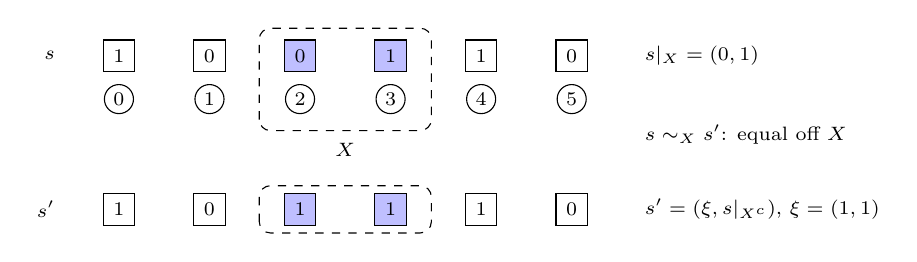
\begin{tikzpicture}[x=1.15cm,y=1cm,
  site/.style={circle,draw,fill=white,inner sep=1.6pt,font=\scriptsize},
  letter/.style={draw,rectangle,inner sep=2pt,minimum size=0.4cm,font=\scriptsize},
  onX/.style={draw,rectangle,inner sep=2pt,minimum size=0.4cm,font=\scriptsize,fill=Blue!25},
  region/.style={rounded corners=4pt,draw,dashed,fill=none},
  lab/.style={font=\scriptsize}]
  % configuration s
  \node[lab,anchor=east] at (-0.6,0.55) {$s$};
  \foreach \u/\l in {0/1,1/0,4/1,5/0} { \node[letter] at (\u,0.55) {\l}; }
  \node[onX] at (2,0.55) {0}; \node[onX] at (3,0.55) {1};
  \foreach \u in {0,...,5} { \node[site] at (\u,0) {\u}; }
  \draw[region] (1.55,-0.4) rectangle (3.45,0.9);
  \node[lab] at (2.5,-0.65) {$X$};
  % configuration s'
  \node[lab,anchor=east] at (-0.6,-1.4) {$s'$};
  \foreach \u/\l in {0/1,1/0,4/1,5/0} { \node[letter] at (\u,-1.4) {\l}; }
  \node[onX] at (2,-1.4) {1}; \node[onX] at (3,-1.4) {1};
  \draw[region] (1.55,-1.7) rectangle (3.45,-1.1);
  \node[lab,anchor=west] at (5.7,0.55) {$s|_X=(0,1)$};
  \node[lab,anchor=west] at (5.7,-1.4) {$s'=(\xi,s|_{X^c})$, $\xi=(1,1)$};
  \node[lab,anchor=west] at (5.7,-0.45) {$s\sim_Xs'$: equal off $X$};
\end{tikzpicture}

\caption{\vet{Two configurations of a chain of six sites with the alphabet $\{0,1\}$, split by
the region $X=\{2,3\}$. They agree off $X$ (the white boxes), so $s\sim_Xs'$, and $s'$ is
$(\xi,s|_{X^c})$ for the letters $\xi=(1,1)$ on $X$. A matrix local to $X$ has a nonzero entry at
$(s,s')$ only for such pairs, and the entry depends on the shaded parts $s|_X$, $s'|_X$ alone
(Definition~\ref{def:localmatrix}).}}
\label{fig:configsplit}
\end{figure}

\begin{definition}[local algebra]\label{def:localmatrix}
\vet{A matrix $M\in\Mat_\Lambda$ is \emph{local to $X$} if
\begin{enumerate}[label=(\arabic*),nosep]
\item $M_{ss'}=0$ whenever $s\not\sim_Xs'$, and
\item $M_{ss'}=M_{rr'}$ whenever $s\sim_Xs'$, $r\sim_Xr'$, $s|_X=r|_X$ and $s'|_X=r'|_X$.
\end{enumerate}
$\cA(X)$ is the set of matrices local to $X$. For a matrix $m$ on the letters of $X$, its
\emph{embedding} $\iota_Xm$ is the matrix $(\iota_Xm)_{ss'}:=\ind{s\sim_Xs'}\,m_{s|_X,s'|_X}$ (the
tensor factor $m\otimes1$ of the sources).}
\end{definition}

\vet{Condition (1) says that $M$ does not change the letters outside $X$; condition (2) that
what it does inside $X$ does not depend on the letters outside. Together they say that $M$ acts
on the part inside $X$ and as the identity outside, which is what $m\otimes1$ means in the
tensor-product picture; the definition avoids the tensor product and keeps every proof an entry
computation. The embedded matrices are exactly the local ones.}

\begin{lemma}[sum over a class]\label{lem:glue}
\vet{For a configuration $s$ and a function $f$ of configurations that vanishes off the class of
$s$ (that is, $f(s')=0$ unless $s'\sim_Xs$),
\begin{equation}\label{eq:glue}
  \sum_{s'}f(s')=\sum_{\xi}f(\xi,s|_{X^c}),
\end{equation}
the right side summing over the choices of letters on $X$.}
\end{lemma}

\begin{proof}
\vet{$\xi\mapsto(\xi,s|_{X^c})$ is a bijection from the letters on $X$ onto the class of $s$,
with inverse $s'\mapsto s'|_X$; re-index the sum, dropping the vanishing terms.}
\end{proof}

\needspace{10\baselineskip}
\begin{proposition}[local algebras]\label{prop:localalgebra}
\begin{enumerate}[label=(\alph*),nosep]
\item \vet{$\cA(X)$ is a star subalgebra of $\Mat_\Lambda$ containing $1$, and it is closed.}
\item \vet{$\iota_Xm\in\cA(X)$, and every $M\in\cA(X)$ is $\iota_Xm$ for \vetnew{some matrix
  $m$ on the letters of $X$}.}
\item \vet{If $X\subseteq Y$ then $\cA(X)\subseteq\cA(Y)$; and $\cA(\Lambda)=\Mat_\Lambda$.}
\end{enumerate}
\end{proposition}

\begin{proof}
\vet{\begin{enumerate}[label=(\alph*),nosep]
\item Both conditions are linear in $M$, hold for $1$ (equal configurations agree off $X$, and
for $s\sim_Xs'$ the equality $s=s'$ is decided by $s|_X=s'|_X$), and are symmetric under
$(s,s')\mapsto(s',s)$, which handles the adjoint. For the product let $M,N\in\cA(X)$. If
$s\not\sim_Xs''$, every term $M_{ss'}N_{s's''}$ vanishes, since $M_{ss'}\ne0$ forces $s'\sim_Xs$
and $N_{s's''}\ne0$ forces $s''\sim_Xs'$. If $s\sim_Xs''$, Lemma~\ref{lem:glue} gives
$(MN)_{ss''}=\sum_\xi M_{s,(\xi,s|_{X^c})}N_{(\xi,s|_{X^c}),s''}$, and each factor is unchanged
when $(s,s'')$ is replaced by $(r,r'')$ with $r\sim_Xr''$ and the same parts on $X$, by
condition (2). Closedness: a subspace of a finite-dimensional space.
\item The embedding satisfies (1) by its indicator and (2) because its entries depend on the
parts on $X$ only. Conversely, \vetnew{fix a configuration $s_0$, which exists as the alphabets
are nonempty, and put $m_{\xi\eta}:=M_{(\xi,s_0|_{X^c}),(\eta,s_0|_{X^c})}$. For} $s\sim_Xs'$
condition (2) with $r=(s|_X,s_0|_{X^c})$,
$r'=(s'|_X,s_0|_{X^c})$ gives $M_{ss'}=m_{s|_X,s'|_X}$, and both sides vanish otherwise.
\item If $s\not\sim_Ys'$ then $s\not\sim_Xs'$. For (2), if $s\sim_Xs'$ then $r\sim_Xr'$, because
off $Y$ the pair $(r,r')$ agrees and on $Y\setminus X$ it copies $(s,s')$, which agrees there;
the restrictions to $X$ agree, so condition (2) for $X$ applies. If $s\not\sim_Xs'$ then
likewise $r\not\sim_Xr'$ and both entries vanish. For $X=\Lambda$ both conditions are empty.\qedhere
\end{enumerate}}
\end{proof}

\begin{theorem}[the qudit net is causal]\label{thm:quditnet}
\vet{$X\mapsto\cA(X)$ is a net over the subsets of $\Lambda$, and local matrices of disjoint
regions commute: $M\in\cA(X)$, $N\in\cA(Y)$ and $X\cap Y=\emptyset$ give $MN=NM$.}
\end{theorem}

\begin{proof}
\vet{Fix $s,s''$. A term $M_{ss'}N_{s's''}$ is nonzero only if $s'$ agrees with $s$ off $X$ and
with $s''$ off $Y$; as $X\cap Y=\emptyset$ this determines $s'$: on $X$ it equals $s''$, elsewhere
$s$. Call it $\bar s$; then $(MN)_{ss''}=M_{s\bar s}N_{\bar ss''}$. Likewise
$(NM)_{ss''}=N_{s\hat s}M_{\hat ss''}$ with $\hat s$ equal to $s''$ on $Y$ and to $s$ elsewhere.
If $s$ and $s''$ differ somewhere off $X\cup Y$, then $\bar s\not\sim_Ys''$ and $\hat s\not\sim_Xs''$,
so both products vanish. Otherwise $M_{s\bar s}=M_{\hat ss''}$ by condition (2) for $X$
($s\sim_X\bar s$, $\hat s\sim_Xs''$, $s|_X=\hat s|_X$, $\bar s|_X=s''|_X$) and
$N_{\bar ss''}=N_{s\hat s}$ by (2) for $Y$, and the two products agree.}
\end{proof}

\vet{Two further constructions serve the examples; both are for a
uniform alphabet $\Omega$. For a matrix $m$ on $\Omega$ and a site $u$, the \emph{single-site
operator} $m_u$ acts by $m$ at the site $u$ and trivially elsewhere,
$(m_u)_{ss'}=\ind{s\sim_{\{u\}}s'}m_{s(u),s'(u)}$, the usual notation $\sigma^x_u$ for a Pauli
matrix at a site. It is local to $\{u\}$ (we read both conditions off the formula);
$m_um'_u=(mm')_u$, because the configurations agreeing with $s$ off $u$ are parametrized by
their letter at $u$, so the sum over them is the matrix product at $(s(u),s''(u))$; operators at
distinct sites commute by Theorem~\ref{thm:quditnet}; and for $u\ne v$ and $s\sim_{\{u,v\}}s''$
the one nonzero term of the product gives $(m_um'_v)_{ss''}=m_{s(u),s''(u)}m'_{s(v),s''(v)}$. A
bijection
$\varphi:\Lambda\to\Lambda'$ of site sets, both with the alphabet $\Omega$, induces the
star-isomorphism $M\mapsto M^\varphi$ of the qudit algebras,
$(M^\varphi)_{rr'}:=M_{r\circ\varphi,\,r'\circ\varphi}$ for configurations $r,r'$ of $\Lambda'$
(re-indexing along the bijection $r\mapsto r\circ\varphi$ of configurations, which commutes with
products and adjoints); it carries $\cA(X)$ onto $\cA(\varphi(X))$, since
$r\sim_{\varphi(X)}r'$ iff $r\circ\varphi\sim_Xr'\circ\varphi$ and $r|_{\varphi(X)}$ determines
$(r\circ\varphi)|_X$ and conversely, so that $M$ is local to $X$ iff $M^\varphi$ is local to
$\varphi(X)$, and $\varphi^{-1}$ gives the inverse. This is the covariance a
translation-invariant system on a finite torus needs. \vetnew{On two qubits, $\sigma^x_1$ is not local
to $\{0\}$: the configurations $00$ and $01$ (the letter at the site $0$ written first) differ
at the site $1$, outside $\{0\}$, yet the entry of $\sigma^x_1$ between them is $1$, against
condition~(1). And $\sigma^x_0$, $\sigma^z_0$ do not commute: the net is not trivial.}}

\subsection{The bounds for spin systems}

\begin{definition}[qudit interaction]\label{def:quditinteraction}
\vet{A \emph{qudit interaction} is a finite family $(S_i,m_i)_{i\in I}$ of finite supports and
Hermitian matrices $m_i$ on the letters of $S_i$; its terms $\Phi_i:=\iota_{S_i}m_i$
are self-adjoint and local to $S_i$, so the family is a Hamiltonian family on the qudit net.}
\end{definition}

\needspace{10\baselineskip}
\begin{theorem}[the published bounds for qudits]\label{thm:quditbounds}
\vet{For a qudit interaction, $a\in\cA(X)$, $b\in\cA(Y)$, with the site matrix $h$ of the
strengths $\kappa_i=\norm{\Phi_i}$:
\begin{enumerate}[label=(\roman*),nosep]
\item for all $t\in\R$, the walk bound \eqref{eq:exchangewalk}, and on the finite lattice
  \begin{equation}\label{eq:quditmatrix}
    \norm{\comm{A(t)}b}\le2\norm a\norm b\Bigl(\ind{X\cap Y\ne\emptyset}
    +\sum_{y\in\bd Y}\sum_{x\in X\cap T}\bigl(e^{2|t|h}-1\bigr)_{yx}\Bigr),
  \end{equation}
  and the same with the roles exchanged, the sum over $\bd X\times(Y\cap T)$;
\item for a \vetnew{decay function} $(F,C_F)$ and an $F$-bound $N_F$, for all $t\in\R$,
  \begin{equation}\label{eq:quditdecay}
    \norm{\comm{A(t)}b}\le2\norm a\norm b\Bigl(\ind{X\cap Y\ne\emptyset}
    +\frac{e^{2N_FC_F|t|}-1}{C_F}\min\{\Sigma_F(Y,X),\Sigma_F(X,Y)\}\Bigr);
  \end{equation}
\item with bounded geometry, for $t\ge0$ as stated there, the forms \eqref{eq:geometryform} and
  \eqref{eq:coneform} of Chapter~\ref{sec:closed}.
\end{enumerate}}
\end{theorem}

\begin{proof}
\vet{Theorem~\ref{thm:hamgenerators} puts the interaction, on the causal net of
Theorem~\ref{thm:quditnet}, under the hypotheses of Chapter~\ref{sec:closed} with a contractive
negation; (i) and (ii) are the time-reversed forms with Theorem~\ref{thm:exchange}, the matrix
form by Proposition~\ref{prop:finite} at $|t|$, (iii) the geometric forms.}
\end{proof}

\vet{\vetnew{Equation~\eqref{eq:quditmatrix} is the review's (3.36) \cite{chen-lucas-yin}, with its
constant doubled and the $-1$ that the series proof gives (the review's $\mathcal C$ is half the
supremum, and the identity has no entry between distinct sites), and with the sum restricted to
$\bd Y\times(X\cap T)$;}
\eqref{eq:quditdecay} is Theorem~3.1 of \cite{nsy2019} for time-independent interactions, whose
boundary $\bd_\Phi$ is $\bd$ when each support carries one nonzero term. Two further facts
connect the \vetnew{decay functions} of Chapter~\ref{sec:closed} to the sources' $F$-functions. In
them, \vetnew{$d$ is a distance on $\Lambda$ as in Definition~\ref{def:geometry} ($d(u,u)=0$ and
the triangle inequality, not assumed symmetric)}, and $T'$ ranges over the finite subsets of
$\Lambda$.}

\begin{proposition}[the $F$-norm; weighted decay functions]\label{prop:fnorm}
\begin{enumerate}[label=(\alph*),nosep]
\item \vet{For \vetnew{a decay function $F>0$ on the finite nonempty set $\Lambda$},
  $\norm\Phi_F:=\max_{x,y}h_{xy}/F(x,y)$ is an $F$-bound, and every $F$-bound $N$ satisfies
  $N\ge\norm\Phi_F$.}
\item \vet{If $(F,C_F)$ is a \vetnew{decay function} and $d$ satisfies the triangle inequality, then for
  $\mu\ge0$ the \vetnew{\emph{weighted decay function}} $F_\mu(x,y):=e^{-\mu d(x,y)}F(x,y)$ is a
  \vetnew{decay function} with
  the same constant $C_F$ (the weighted $F$-functions of \cite{nsy2019}, eq.~(3.11), for the
  weight $\mu r$).}
\end{enumerate}
\end{proposition}

\begin{proof}
\vet{\begin{enumerate}[label=(\alph*),nosep]
\item A maximum dominates each value, and $F>0$ clears the denominator; conversely
$h_{xy}/F(x,y)\le N$ for every pair bounds the maximum.
\item $e^{-\mu(d(x,z)+d(z,y))}\le e^{-\mu d(x,y)}$ for $\mu\ge0$, so
\[
\sum_{z\in T'}F_\mu(x,z)F_\mu(z,y)\le e^{-\mu d(x,y)}\sum_{z\in T'}F(x,z)F(z,y)\le C_FF_\mu(x,y).\qedhere
\]
\end{enumerate}}
\end{proof}

\vetnew{With $F(x,y)=F_0(d(x,y))$ and one term per support, the number $\norm\Phi_F$ of (a) is
the $F$-norm $\sup_{x,y}F_0(d(x,y))^{-1}\sum_{Z\ni x,y}\norm{\Phi(Z)}$ of \cite{nsy2019},
eq.~(3.14); with several terms on a support, $h$ adds their norms.}

\vet{\vetnew{The polynomial decay function $F=F_0\circ d$ with $F_0(r)=(1+r)^{-\alpha}$ on
$\Z^\nu$ with the $\ell^1$ distance has $C_F\le2^\alpha\norm F$ for $\alpha>\nu$, where
$\norm F=\sup_x\sum_yF(x,y)$}; this is
eq.~(3.13) of \cite{nsy2019}, quoted here and not derived (the elementary estimate
$(1+d(x,z))(1+d(z,y))\ge\tfrac12(1+d(x,y))(1+\min\{d(x,z),d(z,y)\})$ gives $2^{\alpha+1}\norm F$).
A finite piece of the lattice inherits the \vetnew{decay function} with a constant at most that of
the lattice. With (b) the \vetnew{weighted decay function} $F_\mu$ gives the exponential light cone of \eqref{eq:quditdecay} at the
velocity $2N_{F_\mu}C_F/\mu$, with $N_{F_\mu}$ an $F_\mu$-bound. On a chain of $20$ sites at
$\alpha=2$ the least reproducing constant is $4.20$ against $2^\alpha\norm F=8.43$; on a
$6\times6$ grid at $\alpha=3$ it is $4.46$ against $16.3$.}

\subsection{Two qubits}

\begin{example}[the exact commutator]\label{ex:twoqubit}
\vet{Two qubits, with the Pauli matrices $\sigma^x=\begin{psmallmatrix}0&1\\1&0\end{psmallmatrix}$,
$\sigma^y=\begin{psmallmatrix}0&-\ii\\\ii&0\end{psmallmatrix}$,
$\sigma^z=\begin{psmallmatrix}1&0\\0&-1\end{psmallmatrix}$ at the sites, $\sigma^x_u$ and so on.
Let $H=\sigma^x_0\sigma^x_1$ (the single term with support $\{0,1\}$ and norm $1$),
$a=\sigma^z_0$, $b=\sigma^z_1$. Since $H^2=1$ and $H$ anticommutes with $a$,
\[
  A(t)=e^{\ii tH}ae^{-\ii tH}=a\,e^{-2\ii tH}=a(\cos2t-\ii\sin2t\,H),\qquad
  \comm{A(t)}b=-2\ii\sin2t\;\sigma^y_0\sigma^y_1,
\]
so $\norm{\comm{A(t)}b}=2|\sin2t|$. The bound \eqref{eq:quditmatrix} has
$h=\begin{psmallmatrix}1&1\\1&1\end{psmallmatrix}$, $\bd Y=\{1\}$, $X\cap T=\{0\}$ and
$(e^{2th}-1)_{10}=(e^{4t}-1)/2$, hence $\norm{\comm{A(t)}b}\le e^{4t}-1$: the ratio of the bound
to the exact norm is $1.24$ at $t=0.1$, $2.05$ at $t=0.3$ and $11.1$ at $t=\pi/4$, where the
commutator is largest. The bound is a bound on growth, not on the oscillation that follows.
\vetnew{The system is that of Example~\ref{ex:twosites} with $\sigma^x$ and $\sigma^z$
exchanged; as there, the path-sum bound of Chapter~\ref{sec:master} gives $4t$ for it, while the
walk bound gives $e^{4t}-1$, the price of counting walks in place of paths.}}
\end{example}

\vet{A second route to the same conclusion, that the dynamics bounded in this chapter is not
trivial, avoids the exponential: at $t=0$ the commutator vanishes by causality, and its
derivative there is \vetnew{$\comm{\ii\comm Ha}b=\ii\,c_0c_1$, the product of the single-site
operators of the matrix $c=\sigma^x\sigma^z-\sigma^z\sigma^x=-2\ii\sigma^y$ at the sites $0$
and $1$. By the product formula for single-site operators, its entry at the row configuration
$00$ and the column configuration $11$ is $\ii\,c(0,1)\,c(0,1)=4\ii\ne0$, where $c(0,1)$ is
the entry of the $2\times2$ matrix $c$ in the row $0$ and the column $1$.} A function vanishing at $0$
with a nonzero derivative there is nonzero at some $t>0$; hence there is $t>0$ with
$\comm{A(t)}b\ne0$.}

\subsection*{Notes and references}
\vetnew{\emph{The review's bound for spin systems.} For edge Hamiltonians $H_e$ on a graph, the
review \cite{chen-lucas-yin} puts $h_{uv}=\sum_{e\ni u,v}\norm{H_e}$ (its eq.~(3.35)) and writes
$\mathcal C_{AB}(t)$ for half the supremum of the commutator norm of an evolved unit operator on
the region $A$ with a unit operator on the region $B$ (its eq.~(3.24)); its bound (3.36) reads
\[
  \mathcal C_{AB}(t)\le\sum_{u\in A,\,v\in B}\bigl(e^{2|t|h}\bigr)_{uv}.
\]

Theorem~\ref{thm:quditbounds}(i) gives it. Take the edges as the supports of a qudit
interaction with the terms $H_e$, so that $\kappa_e=\norm{H_e}$ and $h$ is the review's matrix,
and put $X=A$, $Y=B$. Halving \eqref{eq:quditmatrix} at unit $a$, $b$ gives
$\mathcal C_{AB}(t)\le\ind{A\cap B\ne\emptyset}+\sum_{y\in\bd B}\sum_{x\in A\cap T}
(e^{2|t|h}-1)_{yx}$. The entries of $e^{2|t|h}-1=\sum_{k\ge1}(2|t|h)^k/k!$ are nonnegative and
$h$ is symmetric, so the double sum is at most $\sum_{u\in A,v\in B}(e^{2|t|h}-1)_{uv}$, and the
indicator is at most the sum of the entries of the identity over $A\times B$; together these
give (3.36).

\emph{Theorem~3.1 of \cite{nsy2019}.} For an interaction $\Phi$ on a metric space of sites, an
$F$-function $F$ with constant $C_F$ and the $F$-norm $\norm\Phi_F$, the theorem states, for a
time-independent interaction, $A\in\cA_X$, $B\in\cA_Y$ and $X\cap Y=\emptyset$,
\[
  \norm{\comm{\tau_t(A)}B}\le\frac{2\norm A\norm B}{C_F}\bigl(e^{2\norm\Phi_FC_F|t|}-1\bigr)D(X,Y),
\]
with $D(X,Y)$ the smaller of $\sum_{x\in X}\sum_{y\in\bd_\Phi Y}F(d(x,y))$ and
$\sum_{x\in\bd_\Phi X}\sum_{y\in Y}F(d(x,y))$ (their eq.~(3.24)).
Theorem~\ref{thm:quditbounds}(ii) gives it on a finite set of sites: take one term $\Phi(Z)$ per
support, the decay function $(x,y)\mapsto F(d(x,y))$, for which their $C_F$ is a reproducing
constant since finite sums are at most the full ones, and the $F$-bound $\norm\Phi_F$
(Proposition~\ref{prop:fnorm}(a) and the paragraph after it). The boundary $\bd$ is their $\bd_\Phi$, and
$\Sigma_F(Y,X)$, $\Sigma_F(X,Y)$ are at most the two sums of $D(X,Y)$, since they run over the
touched sites only and their $d$ is symmetric.}

\paragraph{Checks.} {\small The algebra of the local matrices and the embedding, the
conjugation form of the dynamics, the two-qubit example (its exact norm, the entries of the
double commutator and the ratios above), the role exchange on a random three-site Hamiltonian,
the $F$-norm and the \vetnew{weighted decay functions} on chains, and the reproducing constants of
the \vetnew{polynomial decay function} on the chain of $20$ sites and the $6\times6$ grid are computed by
\texttt{checks/m2\_check.py}.}
